\chapter{Elementi Orbitali}
\label{ch:elementi_orbitali}

\section{Introduzione agli Elementi Orbitali}

Un \textbf{elemento orbitale} è un parametro che descrive la forma, la dimensione, l'orientamento e la posizione di un'orbita nello spazio. Per il problema dei due corpi, sono necessari esattamente sei parametri per specificare univocamente un'orbita, corrispondenti ai sei gradi di libertà (tre per la posizione, tre per la velocità).

Esistono diversi insiemi di elementi orbitali, ognuno con vantaggi per applicazioni specifiche:
\begin{itemize}
    \item \textbf{Elementi kepleriani}: Classici, geometricamente intuitivi
    \item \textbf{Elementi cartesiani}: Semplici per l'integrazione numerica
    \item \textbf{Elementi equinoziali}: Evitano singolarità a bassa inclinazione
    \item \textbf{Elementi di Delaunay}: Canonici, utili per la teoria delle perturbazioni
\end{itemize}

\section{Elementi Kepleriani Classici}

Gli \textbf{elementi kepleriani classici} sono l'insieme più ampiamente utilizzato. Descrivono direttamente la geometria di un'orbita a sezione conica.

\subsection{I Sei Elementi Kepleriani}

\begin{enumerate}
    \item \textbf{Semiasse maggiore} ($a$): Metà del diametro più lungo dell'ellisse. Determina la dimensione orbitale e il periodo.
    \begin{equation}
        a = \frac{r_{\text{peri}} + r_{\text{apo}}}{2}
    \end{equation}
    Unità: UA (unità astronomiche) per gli asteroidi, km per i satelliti.
    
    \item \textbf{Eccentricità} ($e$): Forma dell'orbita.
    \begin{equation}
        e = \frac{r_{\text{apo}} - r_{\text{peri}}}{r_{\text{apo}} + r_{\text{peri}}}
    \end{equation}
    \begin{itemize}
        \item $e = 0$: Orbita circolare
        \item $0 < e < 1$: Orbita ellittica
        \item $e = 1$: Traiettoria parabolica
        \item $e > 1$: Traiettoria iperbolica
    \end{itemize}
    
    \item \textbf{Inclinazione} ($i$): Angolo tra il piano orbitale e il piano di riferimento (equatore o eclittica).
    \begin{equation}
        0^\circ \leq i \leq 180^\circ
    \end{equation}
    \begin{itemize}
        \item $i < 90^\circ$: Orbita prograda (diretta)
        \item $i = 90^\circ$: Orbita polare
        \item $i > 90^\circ$: Orbita retrograda
    \end{itemize}
    
    \item \textbf{Longitudine del nodo ascendente} ($\Omega$): Angolo dalla direzione di riferimento al nodo ascendente (dove l'orbita attraversa il piano di riferimento andando verso nord).
    \begin{equation}
        0^\circ \leq \Omega < 360^\circ
    \end{equation}
    
    \item \textbf{Argomento del perielio} ($\omega$): Angolo dal nodo ascendente al perielio all'interno del piano orbitale.
    \begin{equation}
        0^\circ \leq \omega < 360^\circ
    \end{equation}
    
    \item \textbf{Anomalia media} ($M$): Posizione del corpo lungo l'orbita in un dato istante, misurata come angolo dal perielio.
    \begin{equation}
        M = n(t - t_{\text{peri}})
    \end{equation}
    dove $n = \sqrt{\mu/a^3}$ è il moto medio.
\end{enumerate}

\begin{figure}[htbp]
\centering
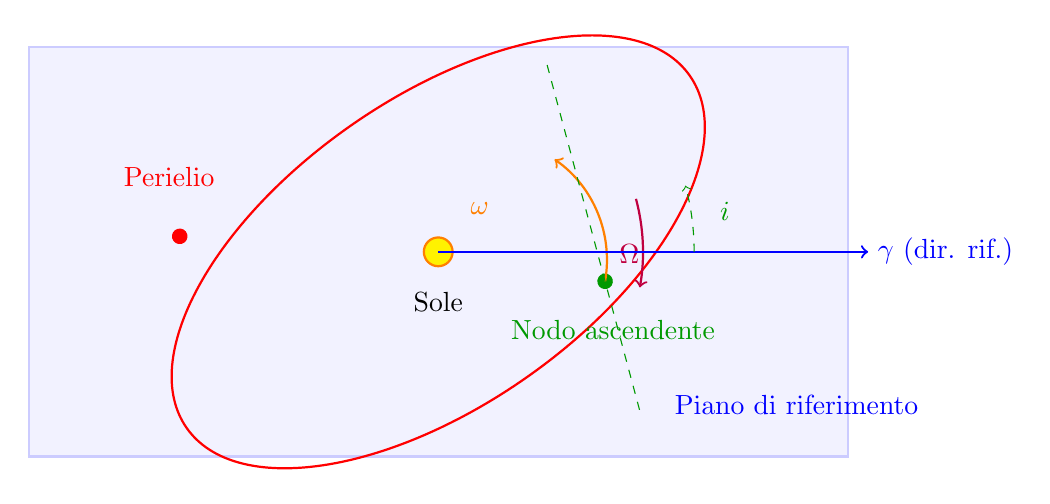
\begin{tikzpicture}[scale=1.3]
    % Piano di riferimento (eclittica o equatore)
    \draw[thick,blue!20,fill=blue!5] (-4,-2) -- (4,-2) -- (4,2) -- (-4,2) -- cycle;
    \node[blue] at (3.5,-1.5) {Piano di riferimento};
    
    % Sole al fuoco
    \filldraw[yellow,draw=orange,thick] (0,0) circle (4pt);
    \node[below] at (0,-0.3) {Sole};
    
    % Piano orbitale (ellisse inclinata)
    \begin{scope}[rotate around={15:(0,0)}]
        % Ellisse
        \draw[thick,red,rotate=20] (0,0) ellipse (3cm and 1.5cm);
        
        % Perielio e afelio
        \filldraw[red] (-2.4,0.8) circle (2pt);
        \node[red,above] at (-2.4,1.2) {Perielio};
        
        % Nodo ascendente
        \filldraw[green!60!black] (1.5,-0.7) circle (2pt);
        \node[green!60!black,below] at (1.5,-1) {Nodo ascendente};
        
        % Longitudine del nodo ascendente (Ω)
        \draw[->,purple,thick] (2,0) arc (0:-25:2);
        \node[purple] at (1.8,-0.5) {$\Omega$};
        
        % Argomento del perielio (ω)
        \draw[->,orange,thick] (1.5,-0.7) arc (-25:40:1.2);
        \node[orange] at (0.5,0.3) {$\omega$};
        
        % Linea inclinazione
        \draw[dashed,green!60!black] (1.5,-2) -- (1.5,1.5);
    \end{scope}
    
    % Direzione di riferimento (punto vernale)
    \draw[->,thick,blue] (0,0) -- (4.2,0);
    \node[blue,right] at (4.2,0) {$\gamma$ (dir. rif.)};
    
    % Angolo di inclinazione
    \draw[->,dashed,green!60!black] (2.5,0) arc (0:15:2.5);
    \node[green!60!black] at (2.8,0.4) {$i$};
\end{tikzpicture}
\caption{Elementi orbitali kepleriani classici. Il piano orbitale (ellisse rossa) è inclinato rispetto al piano di riferimento. Il nodo ascendente è dove l'orbita attraversa il piano di riferimento andando verso nord.}
\label{fig:keplerian_elements_it}
\end{figure}

\subsection{Periodo Orbitale}

Per le orbite ellittiche, la Terza Legge di Keplero mette in relazione il periodo con il semiasse maggiore:
\begin{equation}
    P = 2\pi\sqrt{\frac{a^3}{\mu}}
\end{equation}
dove $\mu = GM$ è il parametro gravitazionale del corpo centrale.

Per il Sole:
\begin{equation}
    P[\text{anni}] = a[\text{UA}]^{3/2}
\end{equation}

Esempi:
\begin{itemize}
    \item Terra: $a = 1$ UA $\Rightarrow P = 1$ anno
    \item Marte: $a = 1.524$ UA $\Rightarrow P = 1.88$ anni
    \item Ceres: $a = 2.77$ UA $\Rightarrow P = 4.61$ anni
\end{itemize}

\subsection{Energia Orbitale}

L'energia orbitale specifica (energia per unità di massa) è:
\begin{equation}
    \mathcal{E} = -\frac{\mu}{2a}
\end{equation}

Si noti che $\mathcal{E} < 0$ per orbite ellittiche (legate), $\mathcal{E} = 0$ per paraboliche e $\mathcal{E} > 0$ per iperboliche.

\subsection{Singolarità degli Elementi Kepleriani}

Gli elementi kepleriani hanno singolarità matematiche:
\begin{itemize}
    \item $\Omega$ non definito per $i = 0^\circ$ (orbita nel piano di riferimento)
    \item $\omega$ non definito per $e = 0$ (orbita circolare, nessun perielio)
    \item Sia $\Omega$ che $\omega$ non definiti per $i = 0^\circ$ ed $e = 0$ simultaneamente
\end{itemize}

Per orbite quasi circolari o quasi equatoriali, gli errori numerici possono diventare grandi. Insiemi di elementi alternativi evitano questi problemi.

\section{Vettore di Stato Cartesiano}

Il \textbf{vettore di stato cartesiano} specifica posizione e velocità in un sistema di riferimento:
\begin{equation}
    \mathbf{X} = \begin{pmatrix} \mathbf{r} \\ \mathbf{v} \end{pmatrix} = \begin{pmatrix} x \\ y \\ z \\ \dot{x} \\ \dot{y} \\ \dot{z} \end{pmatrix}
\end{equation}

\subsection{Vantaggi}
\begin{itemize}
    \item Nessuna singolarità
    \item Equazioni del moto semplici: $\ddot{\mathbf{r}} = -\mu \mathbf{r}/r^3 + \mathbf{a}_{\text{pert}}$
    \item Uso diretto negli integratori numerici
    \item Facile includere perturbazioni
\end{itemize}

\subsection{Svantaggi}
\begin{itemize}
    \item Meno intuitivo degli elementi kepleriani
    \item Difficile interpretare direttamente la geometria orbitale
    \item Sei variabili strettamente accoppiate nell'integrazione
\end{itemize}

\subsection{Conversione: Kepleriano a Cartesiano}

Dati gli elementi kepleriani $(a, e, i, \Omega, \omega, M)$ all'epoca $t_0$:

\textbf{Passo 1}: Risolvere l'equazione di Keplero per l'anomalia eccentrica $E$:
\begin{equation}
    M = E - e\sin E
\end{equation}
(Richiede soluzione iterativa, es. Newton-Raphson)

\textbf{Passo 2}: Calcolare l'anomalia vera $\nu$:
\begin{equation}
    \nu = 2\arctan\left(\sqrt{\frac{1+e}{1-e}}\tan\frac{E}{2}\right)
\end{equation}

\textbf{Passo 3}: Posizione e velocità nel piano orbitale:
\begin{align}
    r &= a(1 - e\cos E) \\
    \mathbf{r}_{\text{orb}} &= r\begin{pmatrix} \cos\nu \\ \sin\nu \\ 0 \end{pmatrix} \\
    \mathbf{v}_{\text{orb}} &= \sqrt{\frac{\mu}{a}}\begin{pmatrix} -\sin E \\ \sqrt{1-e^2}\cos E \\ 0 \end{pmatrix}
\end{align}

\textbf{Passo 4}: Ruotare nel sistema di riferimento usando la matrice di rotazione:
\begin{equation}
    \mathbf{R}_{3}(-\omega)\mathbf{R}_{1}(-i)\mathbf{R}_{3}(-\Omega)
\end{equation}
dove $\mathbf{R}_1(\theta)$ e $\mathbf{R}_3(\theta)$ sono rotazioni attorno agli assi 1 e 3.

\subsection{Conversione: Cartesiano a Kepleriano}

Data la posizione $\mathbf{r}$ e la velocità $\mathbf{v}$:

\textbf{Passo 1}: Calcolare il momento angolare:
\begin{equation}
    \mathbf{h} = \mathbf{r} \times \mathbf{v}
\end{equation}

\textbf{Passo 2}: Calcolare il vettore del nodo:
\begin{equation}
    \mathbf{n} = \mathbf{\hat{z}} \times \mathbf{h}
\end{equation}

\textbf{Passo 3}: Calcolare il vettore di eccentricità:
\begin{equation}
    \mathbf{e}_{\text{vec}} = \frac{1}{\mu}\left[(\mathbf{v} \times \mathbf{h}) - \mu\frac{\mathbf{r}}{r}\right]
\end{equation}

\textbf{Passo 4}: Estrarre gli elementi:
\begin{align}
    a &= \frac{1}{2/r - v^2/\mu} \\
    e &= |\mathbf{e}_{\text{vec}}| \\
    i &= \arccos\frac{h_z}{|\mathbf{h}|} \\
    \Omega &= \arctan\frac{n_y}{n_x} \\
    \omega &= \arccos\frac{\mathbf{n} \cdot \mathbf{e}_{\text{vec}}}{|\mathbf{n}||\mathbf{e}_{\text{vec}}|} \\
    \nu &= \arccos\frac{\mathbf{e}_{\text{vec}} \cdot \mathbf{r}}{|\mathbf{e}_{\text{vec}}||\mathbf{r}|}
\end{align}

Quindi $M = E - e\sin E$ dove $E = 2\arctan\left(\sqrt{\frac{1-e}{1+e}}\tan\frac{\nu}{2}\right)$.

\section{Elementi Equinoziali}

Gli \textbf{elementi equinoziali} evitano singolarità a inclinazione ed eccentricità zero. Sono particolarmente utili per asteroidi con orbite quasi circolari o a bassa inclinazione.

\subsection{Definizione}

L'insieme equinoziale è:
\begin{align}
    a &= \text{semiasse maggiore (uguale al kepleriano)} \\
    h &= e\sin(\omega + \Omega) \\
    k &= e\cos(\omega + \Omega) \\
    p &= \tan(i/2)\sin\Omega \\
    q &= \tan(i/2)\cos\Omega \\
    \lambda &= M + \omega + \Omega \quad \text{(longitudine media)}
\end{align}

\subsection{Conversione a Kepleriano}

Da equinoziale a kepleriano:
\begin{align}
    e &= \sqrt{h^2 + k^2} \\
    i &= 2\arctan\sqrt{p^2 + q^2} \\
    \Omega &= \arctan\frac{p}{q} \\
    \omega &= \arctan\frac{h}{k} - \Omega \\
    M &= \lambda - \omega - \Omega
\end{align}

\subsection{Vantaggi}

\begin{itemize}
    \item Nessuna singolarità per $i \approx 0$ o $e \approx 0$
    \item Evoluzione regolare vicino a orbite circolari/equatoriali
    \item Utilizzato nel sistema HORIZONS di JPL
    \item Ben adatto per la propagazione orbitale numerica
\end{itemize}

\section{Elementi di Delaunay}

Gli \textbf{elementi di Delaunay} sono un insieme canonico di variabili azione-angolo utilizzato nella teoria delle perturbazioni e nella meccanica hamiltoniana.

\subsection{Definizione}

Le variabili di Delaunay sono:
\begin{align}
    L &= \sqrt{\mu a} \quad &\text{(azione coniugata a } \ell = M) \\
    G &= L\sqrt{1-e^2} \quad &\text{(azione coniugata a } g = \omega) \\
    H &= G\cos i \quad &\text{(azione coniugata a } h = \Omega)
\end{align}

Gli angoli sono:
\begin{align}
    \ell &= M \quad \text{(anomalia media)} \\
    g &= \omega \quad \text{(argomento del perielio)} \\
    h &= \Omega \quad \text{(longitudine del nodo ascendente)}
\end{align}

\subsection{Proprietà}

\begin{itemize}
    \item $(L,G,H,\ell,g,h)$ formano un insieme di coordinate canoniche
    \item Formulazione hamiltoniana: $\dot{q}_i = \partial H/\partial p_i$, $\dot{p}_i = -\partial H/\partial q_i$
    \item Hamiltoniana imperturbata: $H_0 = -\mu^2/(2L^2)$ (dipende solo da $L$)
    \item Per il problema di Keplero imperturbato: $L, G, H$ sono costanti
    \item Utile per la teoria delle perturbazioni secolari e l'analisi delle risonanze
\end{itemize}

\section{Implementazione in AstDyn}

AstDyn fornisce funzioni di conversione nella classe \texttt{OrbitalElements}:

\begin{lstlisting}[language=C++,caption={Conversioni di elementi orbitali in AstDyn}]
#include <astdyn/core/OrbitalElements.hpp>
#include <astdyn/core/StateVector.hpp>

using namespace astdyn;

// Elementi kepleriani
OrbitalElements kep;
kep.a = 2.77;        // UA
kep.e = 0.078;
kep.i = 10.6 * DEG_TO_RAD;  // radianti
kep.Omega = 80.3 * DEG_TO_RAD;
kep.omega = 73.1 * DEG_TO_RAD;
kep.M = 15.2 * DEG_TO_RAD;
kep.epoch = 2460000.0;  // JD

// Converti a cartesiano
StateVector sv = kep.to_state_vector();
std::cout << "Posizione: " << sv.r.transpose() << " UA\n";
std::cout << "Velocita: " << sv.v.transpose() << " UA/giorno\n";

// Converti di nuovo a kepleriano
OrbitalElements kep2 = OrbitalElements::from_state_vector(
    sv.r, sv.v, sv.t
);

// Verifica round-trip
std::cout << "Delta a: " << kep2.a - kep.a << " UA\n";
// Output: Delta a: 3.14e-15 UA (precisione macchina)

// Converti a equinoziale
auto eq = kep.to_equinoctial();
std::cout << "h = " << eq.h << ", k = " << eq.k << "\n";
std::cout << "p = " << eq.p << ", q = " << eq.q << "\n";
\end{lstlisting}

\section{Riepilogo}

Punti chiave sugli elementi orbitali:

\begin{enumerate}
    \item Sei parametri specificano un'orbita del problema dei due corpi (6 gradi di libertà)
    \item Gli \textbf{elementi kepleriani} $(a,e,i,\Omega,\omega,M)$ sono geometricamente intuitivi
    \item Lo \textbf{stato cartesiano} $(\mathbf{r}, \mathbf{v})$ è semplice per il lavoro numerico
    \item Gli \textbf{elementi equinoziali} evitano singolarità a $e=0$ e $i=0$
    \item Gli \textbf{elementi di Delaunay} sono canonici, utili per la teoria delle perturbazioni
    \item La scelta degli elementi dipende dall'applicazione e dalle caratteristiche dell'orbita
    \item Le conversioni tra insiemi di elementi sono operazioni standard in AstDyn
\end{enumerate}

Comprendere gli elementi orbitali è essenziale per:
\begin{itemize}
    \item Leggere e interpretare i cataloghi osservativi
    \item Impostare problemi di propagazione orbitale
    \item Analizzare la dinamica e le perturbazioni orbitali
    \item Scegliere metodi numerici appropriati
\end{itemize}

Nel prossimo capitolo, studieremo in dettaglio il problema dei due corpi—il fondamento della meccanica orbitale e la base per tutte le analisi delle perturbazioni.
